\documentclass[a4paper,11pt]{article}
\usepackage[utf8]{inputenc}
\usepackage[spanish]{babel}
%\usepackage[T1]{fontenc}
\usepackage{amsmath}
\usepackage{amssymb}
\usepackage[dvips]{graphicx}
\usepackage{enumerate}
\usepackage{epstopdf}

\topmargin=0cm
\oddsidemargin=0cm
\textheight=23cm
\textwidth=16cm

%opening
\title{\Huge{\textbf{Guía para el Proyecto 6: Esquivador de Obstáculos}}}
\author{Club de Robótica - FI - UNLP}
\date{}

\begin{document}

\maketitle

\section{Introducción}

La idea de la siguiente práctica es lograr familiarizarse con los sensores y actuadores (sensor de proximidad, motores) que conformarían un Esquivador de Obstáculos para su posterior implementación. Para ello se darán una serie de ejercicios que promuevan la utilización de los mismos mediante el Arduino UNO.

Los elementos de circuito que se deben dominar para realizar un esquivador de obstáculos son básicamente:

\begin{itemize}
	\item Motores de corriente continua 
	\item Servomotor
	\item Sensor de proximidad HC-SR04
\end{itemize}
 


\section{Sugerencias para antes de programar}

Para lograr hacer los programas en el Arduino satisfactoriamente es conveniente tener en cuenta previamente los siguientes ítems:

\begin{enumerate}
	\item Tener las nociones básicas de programación en Arduino, así como saber manipular las funciones más utilizadas.	
	\item Conocer los diferentes módulos que dispone el microcontrolador del Arduino (Timmer, ADC, UART).
	\item Segmentar el programa del controlador en subprogramas, para facilitar el desarrollo del mismo.
	\item Implementar los programas en alguno de los prototipos desarrollados por el CDR FI-UNLP.
	\item Contar con los esquemáticos necesarios que describan el pinout de cada placa o shield implementado en el proyecto.
	\item Contar con las hojas de datos de todos los elementos de circuito utilizados.
\end{enumerate}
 
 


\section{Ejercicios para practicar con el Arduino}

\subsection*{Ejercicio 1: Motores de Corriente Continua}Los motores utilizados para la tracción de las ruedas funcionan con tensión continua, y para invertir el giro en los mismos basta con invertir la polaridad de la tensión aplicada. Recordar que el motor izquierdo
está controlado por los pines 3 y 11 del Arduino, mientras que el derecho lo está por los pines 5 y 8.
\begin{itemize}
		\item[a) ] Realizar un programa en Arduino que haga mover al carro en línea recta hacia adelante y luego hacia atrás ciclicamente.
		
		\textbf{Ayuda:} Recordar que los pines que serán salida deberán ser configurados previamente como tales con la instrucción \textbf{pinMode(x,y)}, donde \textbf{x} es el numero de pin a configurar, e \textbf{y} debe ser \textbf{INPUT} (para configurarlo como entrada) u \textbf{OUTPUT} (para configurarlo como salida). Para poner algún valor digital en los pines de salida se utiliza la instrucción \textbf{digitalWrite(x,y)}, donde \textbf{x} es el numero de pin a setear, e \textbf{x} debe ser \textbf{HIGH} (para que sea un 1 lógico) o \textbf{LOW} (para que sea un 0 lógico).
		
		\item[b) ] Realizar un programa en Arduino que haga girar al carro en una circunferencia de un determinado radio.
		
		\textbf{Ayuda:} Para llevarlo a cabo es necesario tener en cuenta que los motores del carro deben girar a velocidades diferentes para efectuar el giro. Para ello es conveniente utilizar señales de PWM y asignar un ancho de pulso distinto en cada motor. Recordar que para generar señales de PWM se utiliza la instrucción \textbf{analogWrite(x,y)}, donde \textbf{x} es el número de pin por donde se quiere sacar la señal PWM, e \textbf{y} es un numero entre 0 y 255 que indica el ciclo de trabajo (0 para el 0\% y 255 para el 100\%) 
\end{itemize}
  


\subsection*{Ejercicio 2: Servomotor}Los servomotores son motores microcontrolados que se caracterizan por poder ubicarse en cualquier posición (dentro de su rango de operación) y mantenerse estable en ella. El servomotor utilizado en el proyecto tiene un ángulo de giro de 180 grados y posee un pin de control a través del cual se lo comanda (la placa shield hecha por el CDR utiliza el pin 9 del Arduino para hacerlo).
\begin{itemize}
		\item[a) ] Realizar un programa en Arduino que haga girar al servomotor desde un extremo del rango de operación hasta el otro, y lo vuelva a hacer ciclicamente.
				
		\textbf{Ayuda:} En la programación en Arduino existen funciones que facilitan enormemente el manejo de los servomotores. La librería \textbf{Servo} contiene todas las funciones necesarias para controlarlo. Para agregar la librería al proyecto basta con añadir una línea al inicio del programa que diga \textbf{\#Include $<$Servo.h$>$}.
		
A continuación se muestra un ejemplo de como utilizar dicha librería:
			
\end{itemize}

	\begin{center}
		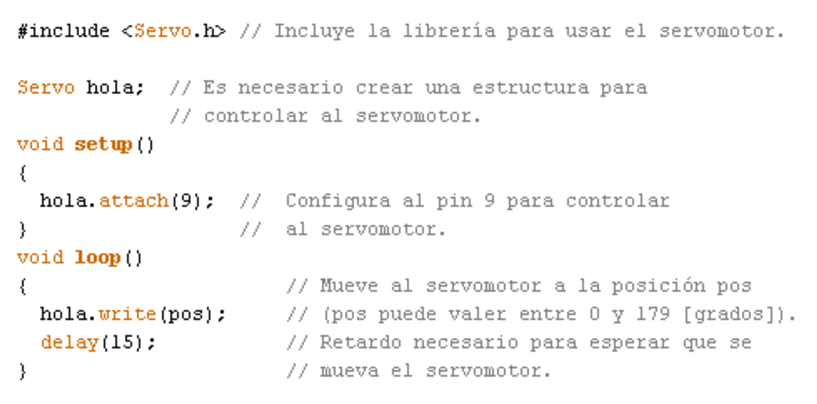
\includegraphics[width=0.8\textwidth]{fig/fig1.eps}
		\begin{center}	
			\textit{Figura 1: Uso de la librería Servo} 
		\end{center}	
	\end{center}



\subsection*{Ejercicio 3: Sensor de proximidad HC-SR04}
El sensor HC-SR04 permite medir la distancia que hay con un determinado objeto a través de pulsos de ultrasonido. Básicamente el funcionamiento consta en enviar pulsos de ultrasonido y esperar a que retorne el eco del mismo. El tiempo que tarda en regresar el eco depende proporcionalmente de la distancia del objeto. El sensor tiene un pin para accionar el mecanismo de sensado (Trigger Input), y otro pin por donde se recibe la información del mismo (Echo Pulse Output):

	\begin{center}
		\includegraphics[width=0.4\textwidth]{fig/fig2.eps}
		\begin{center}		
			\textit{Figura 2: Sensor HC-SR04}
		\end{center}	
	\end{center}


El diagrama de tiempos de la \textit{Figura 3} indica que es necesario enviar un pulso de 10$\mu S$ por el pin Trigger Output para comenzar el sensado, luego el módulo HC-SR04 enviará 8 pulsos de una señal de ultrasonido de 40kHz y esperará el eco. Una vez recibido el eco, el sensor generará un pulso de duración $\Delta t$ en el pin Echo Pulse Output. La relación entre la distancia y el ancho del pulso generado está dada por la relación: 
	
	\begin{center}
		\textit{distancia = $\Delta t$*340$\frac{m}{s}$/2}
	\end{center}

	\begin{center}
		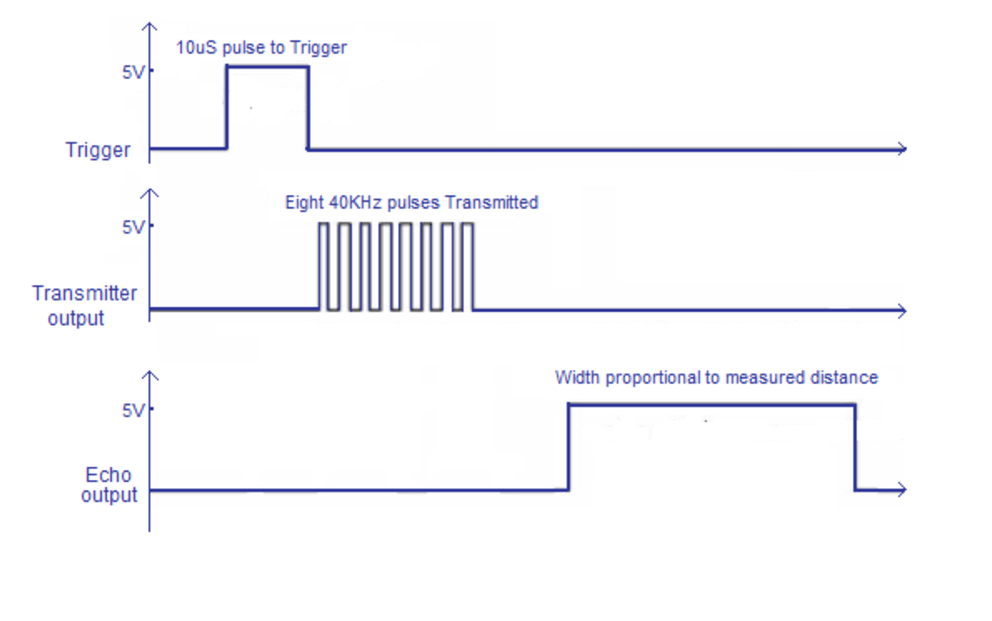
\includegraphics[width=1\textwidth]{fig/fig3.eps}
		\begin{center}	
			\textit{Figura 3: Diagrama temporal de señales para el sensor HC-SR04}
		\end{center}	
	\end{center}

	
\begin{itemize}
	\item[a) ] Realizar un programa en Arduino para medir la distancia que hay entre el sensor y un objeto, y enviarla a la PC a través del puerto serie para poder visualizarla en pantalla.

\textbf{Ayuda:} Para utilizar el sensor fácilmente con Arduino se debe incluir la librería \textbf{Ultrasonic} añadiendo al inicio del programa \textbf{\#Include $<$Ultrasonic.h$>$}. En la \textit{figura 4} se muestra un ejemplo de como utilizar dicha librería:
	\begin{center}
		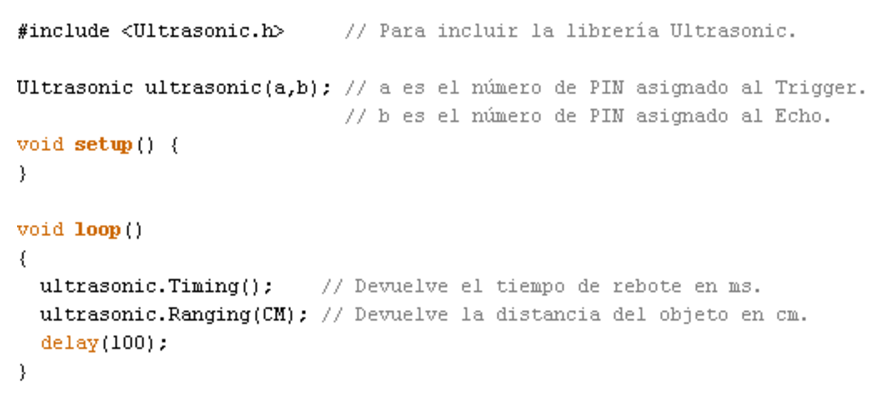
\includegraphics[width=0.9\textwidth]{fig/fig4.eps}
		\begin{center}	
			\textit{Figura 4: Uso de la librería Ultrasonic}
		\end{center}	
	\end{center}


También, para utilizar el módulo UART para la comunicación por el puerto serie se debe utilizar las funciones  \textbf{Serial}. En la figura 5 se muestran las instrucciones más comunes:
\end{itemize}

	\begin{center}
		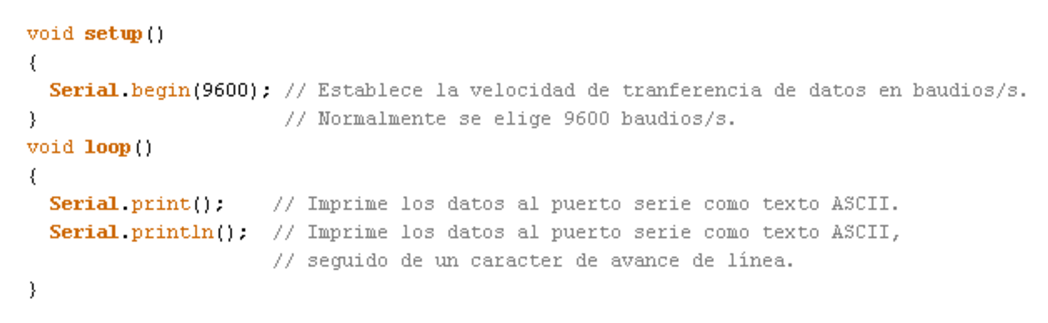
\includegraphics[width=1\textwidth]{fig/fig5.eps}
		\begin{center}	
			\textit{Figura 5: Uso de las funciones Serial}
		\end{center}	
	\end{center}


\end{document}
